\chapter{Introduzione ai Protocolli}
\section{Comunicazione fra host}
\fcolorbox{blue}{white}{\hl{\textbf{Obiettivo:} trasferire un insieme di bit da un host a un altro.}}
\\ 
\vspace*{0.025\textheight}
Bisogna anche assicurare:
\begin{itemize}
    \item \textbf{Massima velocità (\textcolor{red}{Performance}).}
    \item \textbf{Nessun fallimento o malfunzionamento. (\textcolor{red}{Affidabilità}).}
    \item \textbf{\textcolor{red}{Sicurezza} nella comunicazione.}
\end{itemize}

\begin{figure}[!htb]
    \centering
    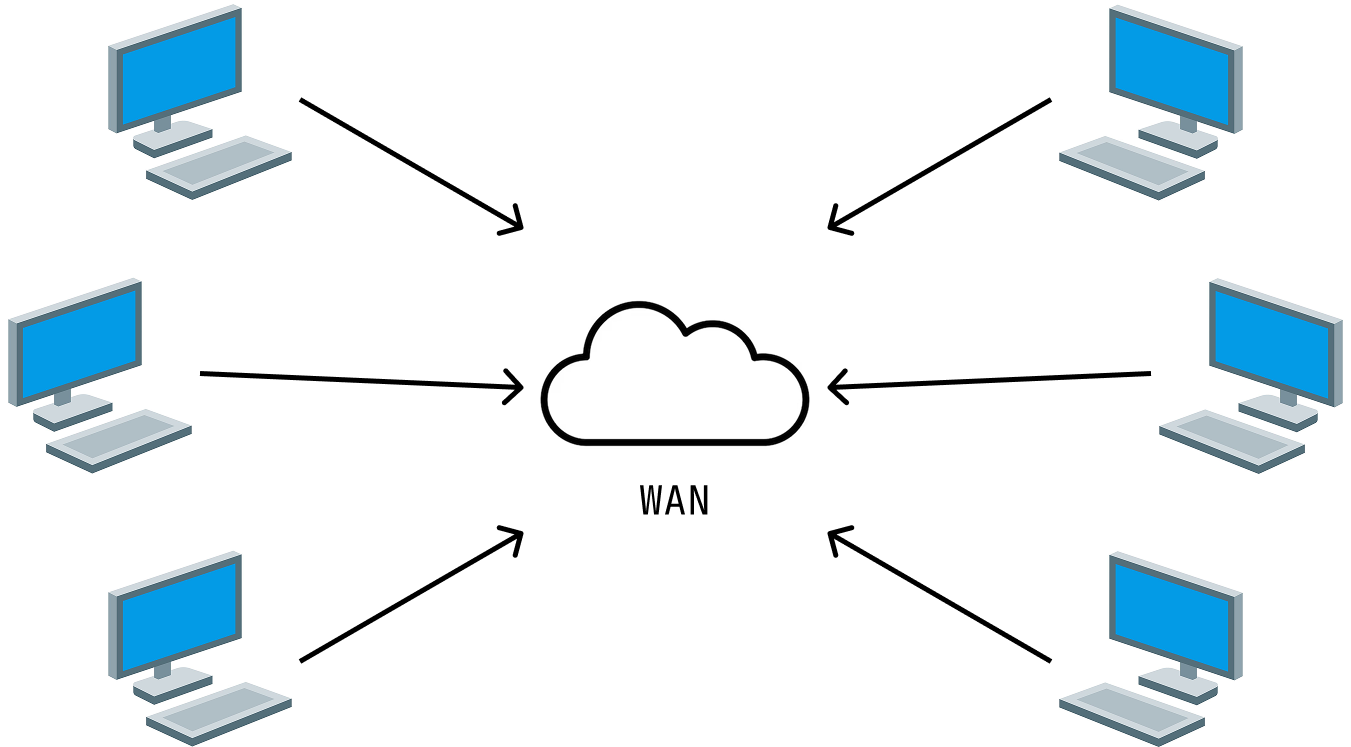
\includegraphics[width=0.5\linewidth]{Images/Protocols/Comunication.png}
    \caption{Comunicazione fra Host}
\end{figure}

\section{Metodologia per comunicare}
La comunicazione, da molto semplice, può diventare complessa. Un modo per nascondere la complessità è l'\textbf{astrazione}. Un modo è dividere l'infrastruttura di rete in diversi \textbf{layer}.

\begin{figure}[!htb]
    \centering
    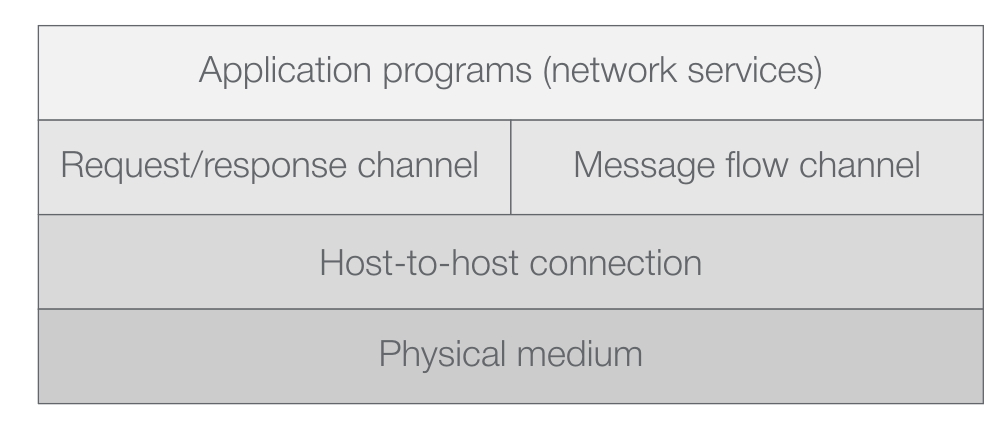
\includegraphics[width=0.6\linewidth]{Images/Protocols/Layers.png}
    \caption{Esempio di layers.}
    \label{fig:layers}
\end{figure}

\newpage
\section{Protocolli}
Le comunicazione richiedono collaborazione e cooperazione per arrivare ad un obiettivo comune, ossia dei \textbf{protocolli} da seguire.

\begin{boxDef}
\textcolor{brown}{\textbf{Protocollo:}} insieme di regole e convenzioni seguite da entità, situate su nodi distinti, che intendono comunicare per svolgere un compito comune.
\end{boxDef}

Ogni protocollo è formato da più parti, tutte utili alla comunicazione:
\begin{enumerate}
    \item \textbf{\textcolor{blue}{Sintassi}:} insieme e strattura di comandi, risposte e formato del messaggio.
    \item \textbf{\textcolor{blue}{Semantica}:} significato dei comandi, delle azione e delle risposte quando trasmetti e ricevi messaggi.
    \item \textbf{\textcolor{blue}{Timing}:} specificazione delle sequenze temporali per comandi, messaggi e risposte.
\end{enumerate}

Comunicazioni complesse richiedono, comunque, l'utilizzo di più protocolli che cooperano fra di loro. I protocolli sono i mattoni di ogni infrastrttura di rete, come l'esempio nella figura \textbf{\ref{fig:layers}}.

Ogni protocollo ha tre interfaccie: 
\begin{enumerate}
    \item Due interfaccie interne per comunicare con il livello superiore e con quello inferiore.
    \item Una interfaccio esterna per comunicare con il protocollo di pari livello di un altro nodo.
\end{enumerate}

\begin{figure}[!htb]
    \centering
    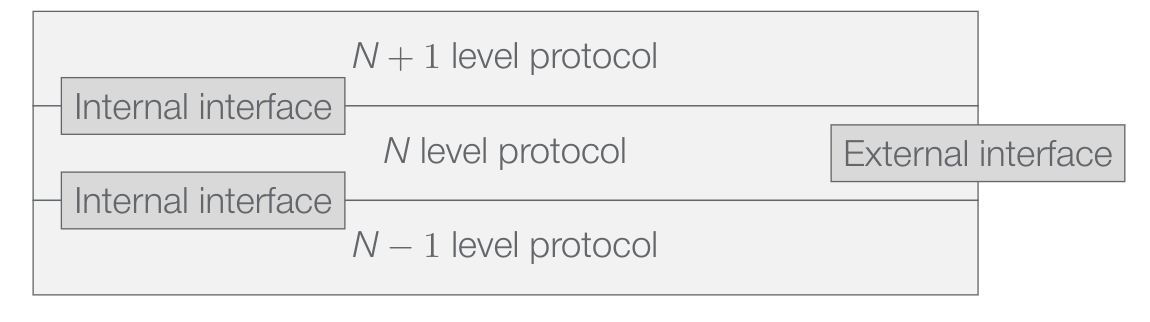
\includegraphics[width=0.6\linewidth]{Images/Protocols/Stack.png}
    \caption{Esempio di comunicazione fra protocolli.}
\end{figure}

\subsection{Protocol Data Unit (PDU)}
Ad ogni livello il messaggio consiste in due parti:
\begin{enumerate}
    \item \textbf{Protocol Control Information (PCI):} ossia l'header.
    \item \textbf{Service Data Unit (SDU):} ossia le informazioni.
\end{enumerate}
L'insieme di queste due parti è il \textbf{PDU}.

\begin{figure}[!htb]
    \centering
    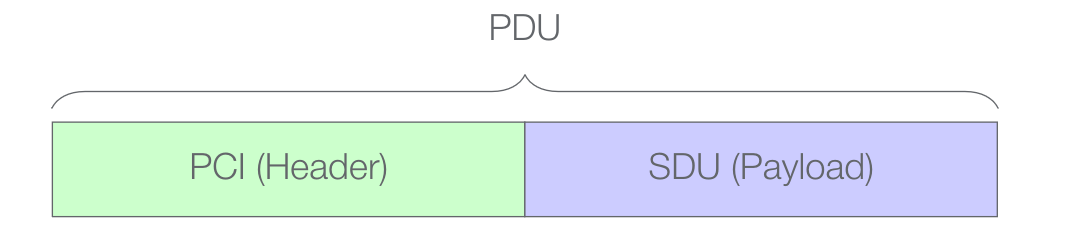
\includegraphics[width=0.6\linewidth]{Images/Protocols/PDU.png}
    \caption{PDU.}
\end{figure}

Ad ogni layer viene incapsulato un header alle informazione, partendo dal livello N fino al livello 1. Successivamente, sarà spacchettato e usato dall'altro host. La gerarchia dei protocolli è definita dall'archittetura dell'infrastruttura di rete a layer.